% renamed file to z5labpic.tex 2013.02.25 and use standalone class
% zn: 2010.3.11 tikzcreatedpdf.tex
% check out Externalization Library in the pgf-tikz manual v2.0

%--------------------------------------------------------------------------
\documentclass
%{article}
{standalone}
%--------------------------------------------------------------------------
\usepackage{tikz}
	\usetikzlibrary{calc}
	\usetikzlibrary{circuits.ee.IEC}
%	\usetikzlibrary{shapes,decorations,shadows}
%	\usetikzlibrary{decorations.pathmorphing}
%	\usetikzlibrary{decorations.shapes}
%	\usetikzlibrary{decorations.text}
%	\usetikzlibrary{fadings}
%	\usetikzlibrary{fit,chains}
%	\usetikzlibrary{patterns}
	\usetikzlibrary{positioning}
%	\usetikzlibrary{decorations.footprints}
%	\usetikzlibrary{decorations.fractals}
	\usetikzlibrary{scopes}
%	\usetikzlibrary{shapes.gates.logic.IEC}
%	\usetikzlibrary{shapes.gates.logic.US}
%	\usepgflibrary{shapes}
\usepackage{pgfplots}
\usepackage{shortvrb} \MakeShortVerb{\"}
\usepackage{multicol} 
\usepackage{verbatim}
%--------------------------------------------------------------------------
\begin{document}
%--------------------------------------------------------------------------
% 3 resistors in series
%\begin{tikzpicture}[circuit ee IEC,set resistor graphic=var resistor IEC graphic]
%	\draw (0,0)
%		to[resistor={info'=$R_1$}]			(1.5,0)
%		to[resistor={info'=$R_2$}]			(3.5,0)
%		to[resistor={info'=$R_3$}]			(5,0);
%\end{tikzpicture}
%\hfill
%\begin{tikzpicture}[circuit ee IEC,set resistor graphic=var resistor IEC graphic]
%	\draw (0,0)
%		to[resistor={info'=$R_1$}]			(2,0)
%		to[resistor={info'=$R_2$}]			(4,0)
%		to[resistor={info'=$R_3$}]			(6,0);
%\end{tikzpicture}
%\hfill
% 3 resistors in parallel
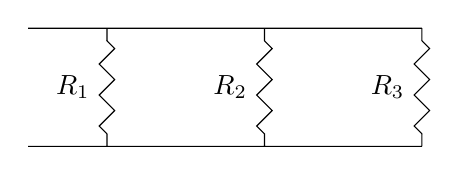
\begin{tikzpicture}[circuit ee IEC,set resistor graphic=var resistor IEC graphic]
	\draw (0,0) to[resistor={info=$R_1$}]	(0,1.5)
		(2,1.5 ) to[resistor={info'=$R_2$}]		(2,0)
		(4,1.5) to[resistor={info'=$R_3$}]		(4,0)
		(-1,0) -- (4,0)
		(-1,1.5) -- (4,1.5);
\end{tikzpicture}


%--------------------------------------------------------------------------
\end{document}
%--------------------------------------------------------------------------

%----voltmeters
\begin{comment}	% battery + resistor
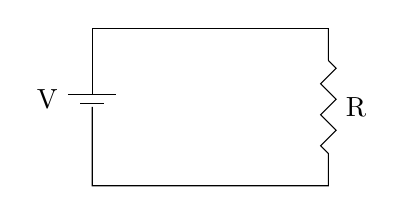
\begin{tikzpicture}[circuit ee IEC,set resistor graphic=var resistor IEC graphic]
	\node (V1) [battery={info'=V},point down] at (0,0.1) {};
%	\draw (0,1) to[make contact={info'=S}]	(2,1)
	\draw (0,1)--(3,1);
	\draw (3,1)	to[resistor={info=R},point down]	(1,3) -- (0,-1) -- (0,0);
	\draw (2,1) -- (3,1); \draw (V1) -- (0,1);
\end{tikzpicture}
\end{comment}
